\chapter{FRICTION AT ICE-I$_\mathrm{h}$ / WATER INTERFACES IS GOVERNED
  BY SOLID / LIQUID HYDROGEN-BONDING}\label{chap:Friction}

% Write a short introduction to the topic discussed in this chapter.
In this chapter, calculations of solid-liquid friction at
ice-I$_\mathrm{h}$ / water interfaces are discussed.  An expression
for friction coefficients appropriate for negative slip boundary
conditions is presented, and the computed friction of these interfaces
is found to be invariant to the shear rate and direction of shear
relative to the surface features. Solid / liquid hydrogen bonds are
identified using local tetrahedral ordering of the water molecules,
and the surface density of these hydrogen bonds is found to directly
correlate with interfacial friction. Surface topography of the
investigated crystal facets at the ice-I$_\mathrm{h}$ / water
interface is quantified by querying mean projected densities. However,
the dimensions of the surface features do not strongly correlate with
the obtained friction coefficients, leading to the conclusion that
friciton is dominated by the density of solid / liquid hydrogen
bonds.  Lastly, we present a simple momentum transmission model using
the density of solid / liquid hydrogen bonds, the shear viscosity of
the liquid, and the structural width of the interface. This model
agrees well with our observed results for both the SPC/E and TIP4P/Ice
simulations. 
%\end{abstract}



%\section{Coefficient of Friction of the Interface}
% As liquid water flows over an ice interface, there is a distance from
% the structural interface where bulk-like hydrodynamics are recovered.
% Bocquet and Barrat constructed a theory for the hydrodynamic boundary
% parameters, which include the slipping length
% $\left(\delta_\mathrm{wall}\right)$ of this boundary layer and the
% ``hydrodynamic position'' of the boundary
% $\left(z_\mathrm{wall}\right)$.\cite{PhysRevLett.70.2726,PhysRevE.49.3079}
% This last parameter is the location (relative to a solid surface)
% where the bulk-like behavior is recovered.  Work by Mundy {\it et al.}
% has helped to combine these parameters into a liquid-solid friction
% coefficient, which quantifies the resistance to pulling the solid
% interface through a liquid,\cite{Mundy1997305}
% \begin{equation}
% \lambda_\mathrm{wall} = \frac{\eta}{\delta_\mathrm{wall}}.
% \end{equation}
% This expression is nearly identical to one provided by Pit {\it et
%   al.} for the solid-liquid friction of an interface,\cite{Pit1999}
% \begin{equation}\label{Pit}
%   \lambda=\frac{\eta}{\delta}
% \end{equation}
% where $\delta$ is the slip length for the liquid measured at the
% location of the interface itself.  In our simulations, the shoulder on
% the velocity profile indicating the location of the hydrodynamic
% boundary in the liquid is not always apparent. In some cases, the
% linear behavior persists nearly up to the interfacial region.  For
% this reason, the hydrodynamic position of the boundary is not always
% computable, while the Pit approach (Eq. \ref{Pit}) can be used to find
% the solid-liquid friction coefficient more reliably.

% In both the Pit and hydrodynamic boundary expressions, $\eta$ is the
% shear viscosity of the bulk-like region of the liquid, a quantity
% which is easily obtained in VSS-RNEMD simulations by fitting the
% velocity profile in the region far from the surface.\cite{Kuang2012}
% Assuming linear response in the bulk-like region,
% \begin{equation}\label{Kuang}
% j_{z}(p_{x})=-\eta \left(\frac{\partial v_{x}}{\partial z}\right)
% \end{equation}
% Substituting this result into eq. \eqref{Pit}, we can estimate the
% solid-liquid friction coefficient using the slip length,
% \begin{equation}
% \lambda=-\frac{j_{z}(p_{x})} {\left(\frac{\partial v_{x}}{\partial
%       z}\right) \delta}.
% \end{equation}

% For ice / water interfaces, the boundary conditions are no-slip, so
% projecting the bulk liquid state velocity profile yields a negative
% slip length. This length is the difference between the structural edge
% of the ice (determined by the tetrahedrality profile) and the location
% where the projected velocity of the bulk liquid intersects the solid
% phase velocity (see Figure \ref{fig:delta_example}). The coefficients
% of friction for the basal and the prismatic facets were determined for
% shearing along both the $x$ and $y$ axes.  The values are given in
% Table \ref{tab:lambda}. 

% Note that the measured friction coefficient for the basal face is
% twice that of the prismatic face (regardless of drag direction).
% These results may seem surprising as the basal face appears smoother
% than the prismatic with only small undulations of the oxygen
% positions, while the prismatic surface has deep corrugated channels
% along the $x$ direction in the crystal system used in this work.
% However, the corrugations are relatively thin, and the liquid phase
% water does not appear to populate the channels.  The prismatic face
% therefore effectively presents stripes of solid-phase molecules
% (making up approximately half of the exposed surface area) with nearly
% empty space between them. The interfacial friction appears to be
% independent of the drag direction, so flow parallel to these channels
% does not explain the lower friction of the prismatic face.  A more
% likely explanation is that the effective contact between the liquid
% phase and the prismatic face is reduced by the empty corrugations.  


\section{Solid-Liquid Friction at Ice-I$_\mathrm{h}$ / Water Interfaces}
In no-stick boundary conditions, fluid flowing over a solid is
characterized by a slip length, $\delta$, describing the extent of
slip of the fluid at the interface. This length is the extrapolated
distance from the interface where the tangential velocity component
vanishes. For solids with weak interactions with the liquid, there is
little drag imposed on the fluid and the resulting interfacial liquid
velocity, $\Delta v_\mathrm{slip}$, can be significant. In no-stick
boundaries, therefore, the extrapolated slip lengths are also large
(top panel of Figure \ref{fig:slipLengthPlot}).  Balasubramanian and
Mundy have related the slip length to the interfacial friction
coefficient, 
\begin{equation}\label{eq:kappa1}
\lambda = \frac{\eta}{\delta}
\end{equation}
where $\eta$ is the shear viscosity of the
liquid.\cite{Balasubramanian1999} For solids that have strong
interactions with the liquid, a larger frictional drag is imposed on
the fluid at the interface and the resulting slip lengths are
smaller. When the solid / liquid interactions become large enough, the
interface is best described with stick boundary conditions, and the
slip length will vanish (middle panel of
Figure \ref{fig:slipLengthPlot}).


\begin{figure}
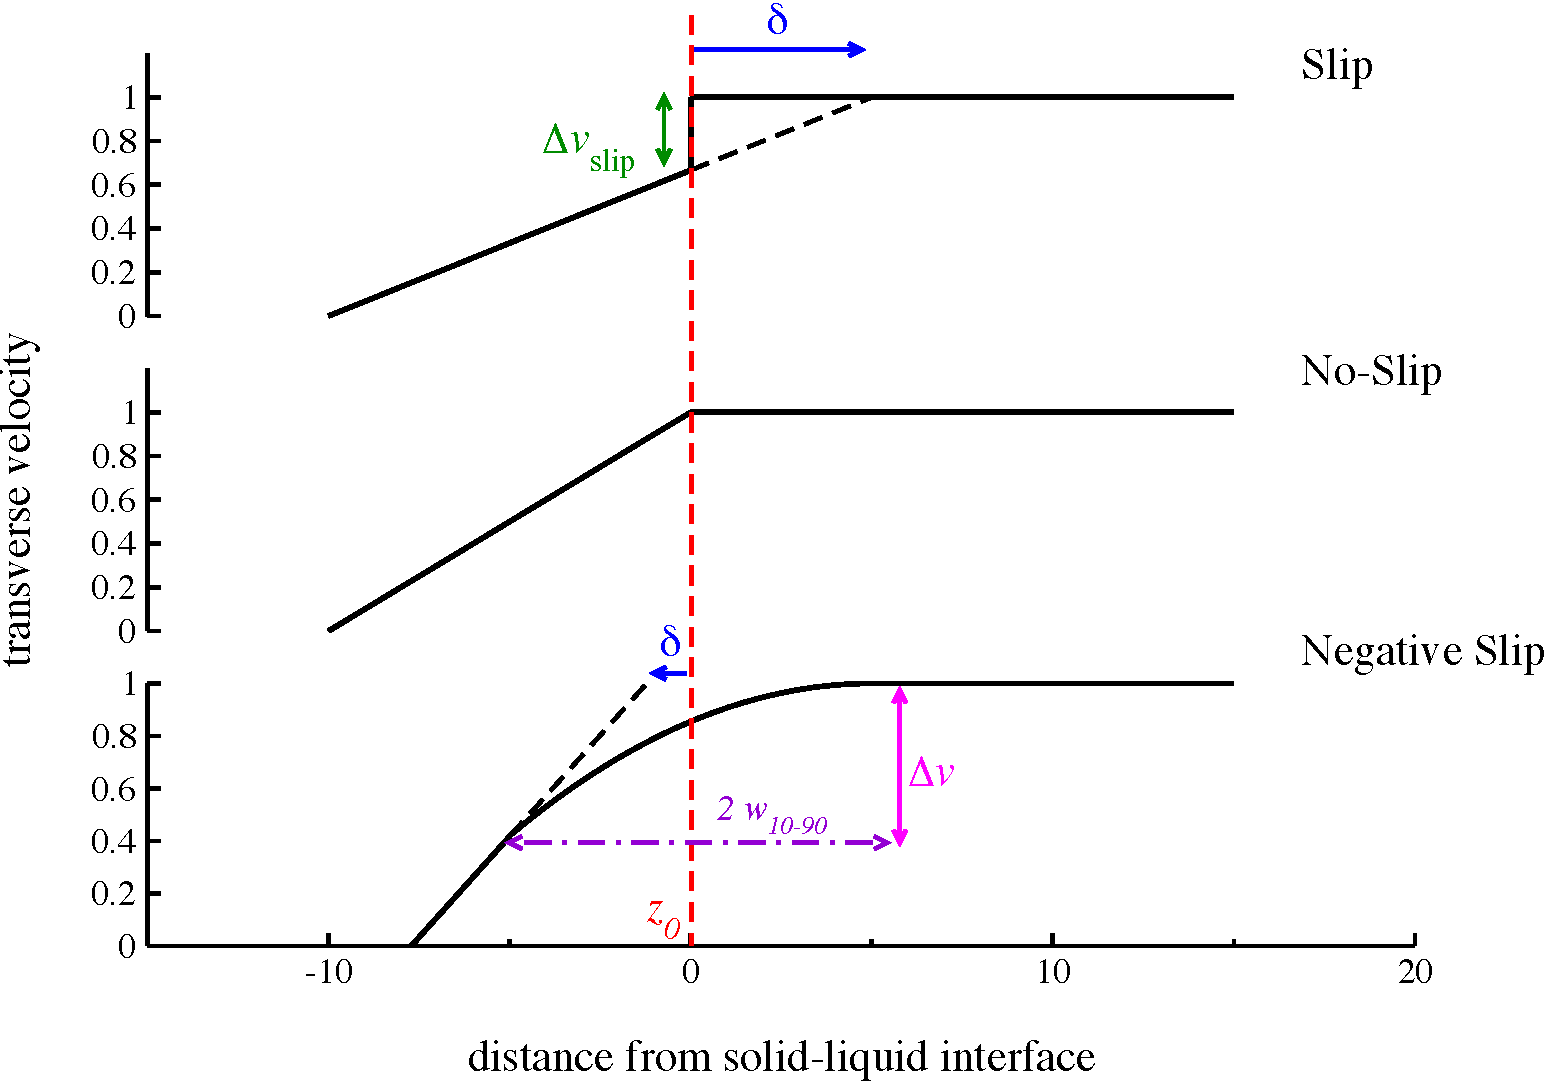
\includegraphics[width=\linewidth]{Figures/slipLengthPlot}
\caption{\label{fig:slipLength} A sketch of transverse velocity
  profiles, $v_x(z)$, for interfaces in slip (top), no-slip (middle),
  and negative slip boundary conditions (bottom).  The location of the
  interface is defined by a Gibbs dividing surface at $z_0$. Under
  negative slip conditions, the 10-90 interfacial width, $w_{10-90}$,
  provides locations that are unambiguously on the liquid and solid
  sides of the interface.\label{fig:slipLengthPlot}}
\end{figure}


In our initial investigation of friction at the basal and prismatic
interfaces,\cite{Louden2013a} we related the interfacial friction
coefficient to the imposed momentum flux $j_z(p_x)$ and the transverse
flow velocity gradient through a linear constitutive relation.
\begin{equation}\label{eq:linConRel}
j_{z}(p_{x})=-\eta \left(\frac{\partial v_{x}}{\partial z}\right)
\end{equation}
Substituting Equation \eqref{eq:linConRel} into Equation \eqref{eq:kappa1} gives
an expression for the friction coefficient in terms of the momentum
flux and the resulting velocity gradient through the liquid region of
the simulation box.
\begin{equation}\label{eq:lambda}
\lambda=-\frac{j_{z}(p_{x})} {\delta\left(\frac{\partial v_{x}}{\partial
      z}\right) }
\end{equation}

For ice-I$_\mathrm{h}$ / water interfaces, the boundary conditions are
no-slip, so projecting the bulk liquid state velocity profile yields a
negative slip length. This length is the difference between the
structural edge of the ice (determined by the tetrahedrality profile)
and the location where the projected velocity of the bulk liquid
intersects the solid phase velocity (see Figure
\ref{fig:delta_example} for a diagram of no-slip conditions at
ice-I$_\mathrm{h}$ / water interfaces). The coefficients of friction
for the basal and prismatic facets were determined for shearing along
both the $x$ and $y$ axes, and are given in Table
\ref{tab:lambda}. The computed friction coefficients were found to be
invariant to shear direction, as $\lambda$ was found to be within
error bars when comparing shearing in either the $x$ or $y$
dimensions. Also we observed that the basal face had about a factor of
two larger friction coefficient as compared to the prismatic
face. Lastly, we note that the computed friction coefficients were
robust under varying shear rates.

\begin{figure}
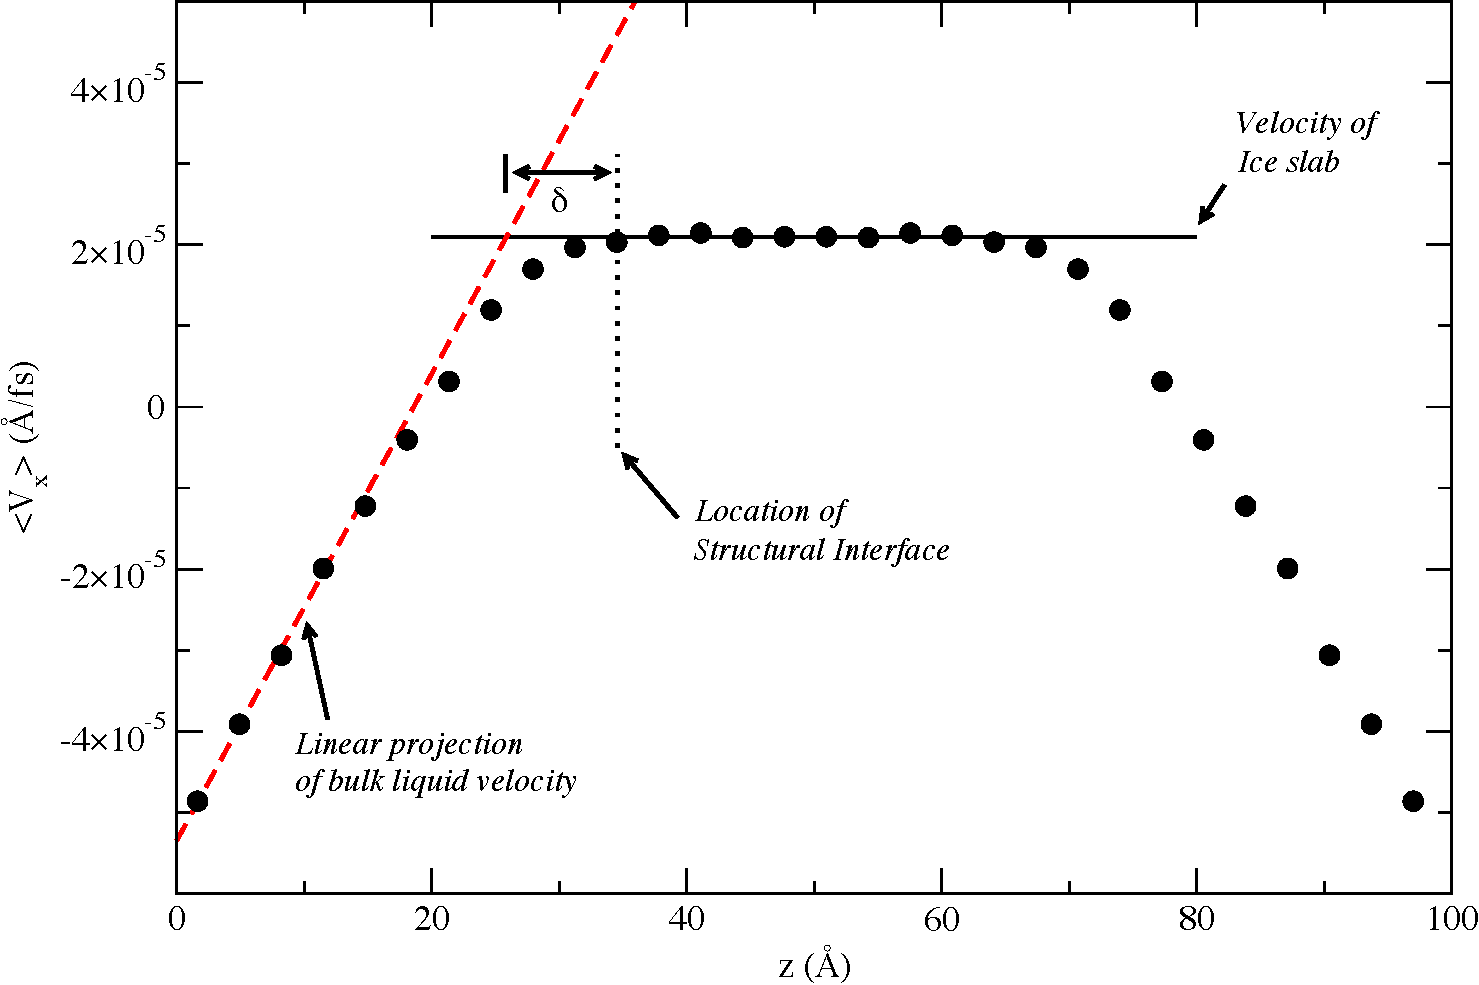
\includegraphics[width=\linewidth]{Figures/delta_example}
\caption{\label{fig:delta_example} Determining the (negative) slip
  length ($\delta$) for the ice-I$_\mathrm{h}$ / water interfaces
  (which have decidedly non-slip behavior).  This length is the
  difference between the structural edge of the ice (determined by the
  tetrahedrality profile) and the location where the projected
  velocity of the bulk liquid (dashed red line) intersects the solid
  phase velocity (solid black line).  The dotted line indicates the
  location of the ice as determined by the tetrahedrality profile.
  This example is taken from the basal-face simulation with an applied
  shear rate of 3.0 ms\textsuperscript{-1}.}
\end{figure}

\begin{table}[h]
\centering
\caption{SOLID-LIQUID FRICTION COEFFICIENTS ($\lambda$) FOR SPC/E
  ICE-I$_\mathrm{h}$ INTERFACES WITH WATER }
\label{tab:lambda}
\begin{tabular}{r|cc}  
\hline
\hline
           & \multicolumn{2}{c}{Drag direction} \\ 
 Interface & $x$               & $y$  \\ \hline
     Basal  $\{0001\}$ &  $0.08 \pm 0.02$  & $0.09 \pm 0.03$ \\
 Prismatic  $\{10\bar{1}0\}$ & $0.037 \pm 0.008$ & $0.04 \pm 0.01$ \\ 
\hline
\hline
\end{tabular}
\begin{flushleft}
  Friction coefficients are measured in
  amu~\AA\textsuperscript{-2}~fs\textsuperscript{-1}.
\end{flushleft}
\end{table}



While this initial investigation provided some insight to friction at
ice-I$_\mathrm{h}$ / water interfaces, stick boundaries pose a problem
for Equation  \eqref{eq:kappa1}, as $\lambda$ asymptotically goes to
infinity as $\delta \rightarrow 0$.  Likewise, some materials (such as
ice-I$_\mathrm{h}$) possess solid / liquid interactions that are
strong enough for the extrapolated tangential velocity to vanish
\textit{before} reaching the solid. The velocity profile yields a
negative slip length as explained above, (bottom panel of Figure
\ref{fig:slipLengthPlot}), and the solid / liquid friction coefficient
defined in Equation \eqref{eq:kappa1} becomes meaningless.  As apparent in
Figure \ref{fig:delta_example}, the tangential velocity profile of the
liquid extrapolates to the solid velocity several molecular layers
before reaching the solid. Thus a new friction coefficient must be
defined to describe these interfaces.

A solid / liquid friction coefficient appropriate for stick
boundaries, $\kappa$, may be defined using the velocity drop
across the interface, rather than the length scale over which this
drop occurs. We can relate the imposed shear stress with the relative
tangential velocity of the fluid in the interfacial
region,\cite{Kuang2012}
\begin{equation}\label{eq:Shenyu-13}
j_{z}(p_{x}) = \kappa_{x} \Delta v
\end{equation}
where $\Delta v = v_{x}(\mathrm{solid}) - v_{x}(\mathrm{liquid})$ is
the difference in transverse velocity between points that are
unambiguously on the solid and liquid sides of the interface.  In slip
boundary conditions, $\kappa$ and $\lambda$ are identical, but
Equation \eqref{eq:Shenyu-13} provides a direct analogy to non-equilibrium
expressions for the interfacial thermal conductance $(G)$,
\begin{equation}
J_z = G~ \Delta T.
\end{equation}
Here, $J_z$ is a thermal flux and the temperature drop is measured
across an interface of \textit{finite width}. By analogy, $\kappa$ is
a transport coefficient that measures \textit{interfacial momentum
  conductance} across an interface of finite width.

At ice-I$_\mathrm{h}$ / water interfaces, the solid / liquid boundary
is not an infinitely thin plane. As we found in Chapters
\ref{chap:Str} and \ref{chap:Dyn}, a large number of order parameters
transitions smoothly between the phases over a few molecular
diameters.  Here, we have used the local tetrahedral order parameter
as the metric for quantifying interfacial width and define locations
in space that are unambiguously on the solid and liquid sides of the
interface. This parameter was chosen due to its ability to
descriminate liquid-like and ice-like water molecules more accurately
than the local density. Also, the computed error bars were
significantly smaller than any of the dynamic order parameters
investigated in Chapter \ref{chap:Dyn}. In what follows, we have used
the Gibbs dividing surface ($z_0$) and the 10$-$90 width of the
interface ($w_\mathrm{10-90}^{q}$) to arrive at physical locations for
measuring $v_{x}(solid)$ and $v_{x}(liquid)$.  These uniquely define a
friction coefficient in terms of well-defined structural features
($z_0$ and $w_\mathrm{10-90}^{q}$) and dynamic properties ($v_{x}(z)$)
of the interface.

Tangential velocity profiles from the simulations were fit using a
piecewise function that is both continuous and continuously
differentiable. The velocity profiles, $v_x(z)$, obtained from each
shearing simulation were fit assuming linear behavior through each of
the three regions of the simulation box; the lower liquid, the solid,
and the upper liquid. Parabolic functions were designed to capture the
negative slip behavior that links the three regions,
\begin{equation}\label{eq:vfit}
v(z) =
\begin{cases}
  v_{l} - m_{l}z & 0 \leq z < (z_{1} - w) \\
  v_{s} - \frac{1}{2}k(z-z_{1})^{2} & (z_{1}-w) \leq z < z_{1} \\
  v_{s}  & z_{1} \leq z < z_{2} \\
  v_{s} - \frac{1}{2}k(z-z_{2})^{2}  & z_{2} \leq z <( z_{2} + w)\\
  v_{s} - \frac{1}{2}kw^{2} - m_{l}(z-(z_{2} + w)) & (z_{2} + w) \leq z \\
\end{cases}
\end{equation}
  
Here, $v_{l}$ is the velocity of the liquid at the middle of the
liquid domain (the edge of the simulation box), and $v_{s}$ is the
velocity of the solid. The locations $z_{1}$ and $z_{2}$ are the edges
of the ice slab, and $w$ is the width of the interface from the
velocity profile (distinct from $w_{10-90}^{q}$). The parameter
$m_{l}$ is the slope of the velocity profile in the liquid regions of
the box which is related to the liquid-state viscosity. Figure
\ref{fig:spComic} shows a representative velocity profile (navy
squares) and fit (green line) with the locations of $z_{1}$ and
$z_{2}$ indicated as vertical dotted lines. Once the fits were
obtained, the values for $v_{x}(\mathrm{solid})$ and $v_{x}(\mathrm{liquid})$ for
Equation \eqref{eq:Shenyu-13} were sampled from the fit. The $z$ locations
used to sample the fit were determined by structural measures. The $z$
location for $v_{x}(\mathrm{liquid})$ was taken to be the Gibbs dividing
surface of the interface, less the 10$-$90 width of the
interface. Similarly, the $z$ location for $v_{x}(\mathrm{solid})$ was taken to
be the Gibbs dividing surface plus the 10$-$90 width of the interface.

\begin{align}
v_{x}(\mathrm{solid}) & = v_{x}( z_0 + w_\mathrm{10-90}^{q})  \label{eq:vx1}\\
v_{x}(\mathrm{liquid}) & = v_{x}( z_0 - w_\mathrm{10-90}^{q}). \label{eq:vx2}
\end{align}
As mentioned earlier, the momentum flux, $j_{z}(p_{x})$ is an imposed
parameter of the VSS-RNEMD simulations, and by using
Equation \eqref{eq:Shenyu-13}, estimates of interfacial friction
coefficient $\kappa$ are straightforward.

The calculated $\kappa$ values found for the four crystalline facets
of ice-I$_\mathrm{h}$ investigated here are shown in Table
\ref{tab:kappa}. Solid / liquid friction coefficients for shearing
simulations where the imposed momentum flux was in the $y$-dimension,
$\kappa_{y}$, are calculated in the same manner, with $j_{z}(p_{y})$
and $v_{y}$ substituting for $j_{z}(p_{x})$ and $v_{x}$ in
Eqs. \eqref{eq:Shenyu-13}, \eqref{eq:vx1}, and \eqref{eq:vx2}.
Similar to our initial results for $\lambda$, these results
for $\kappa$ were found to be independent of the shear rate (see
Figure \ref{fig:kappaPlot}), as well as the direction of the shear
relative to the features on the surfaces of the facets.


\begin{figure}
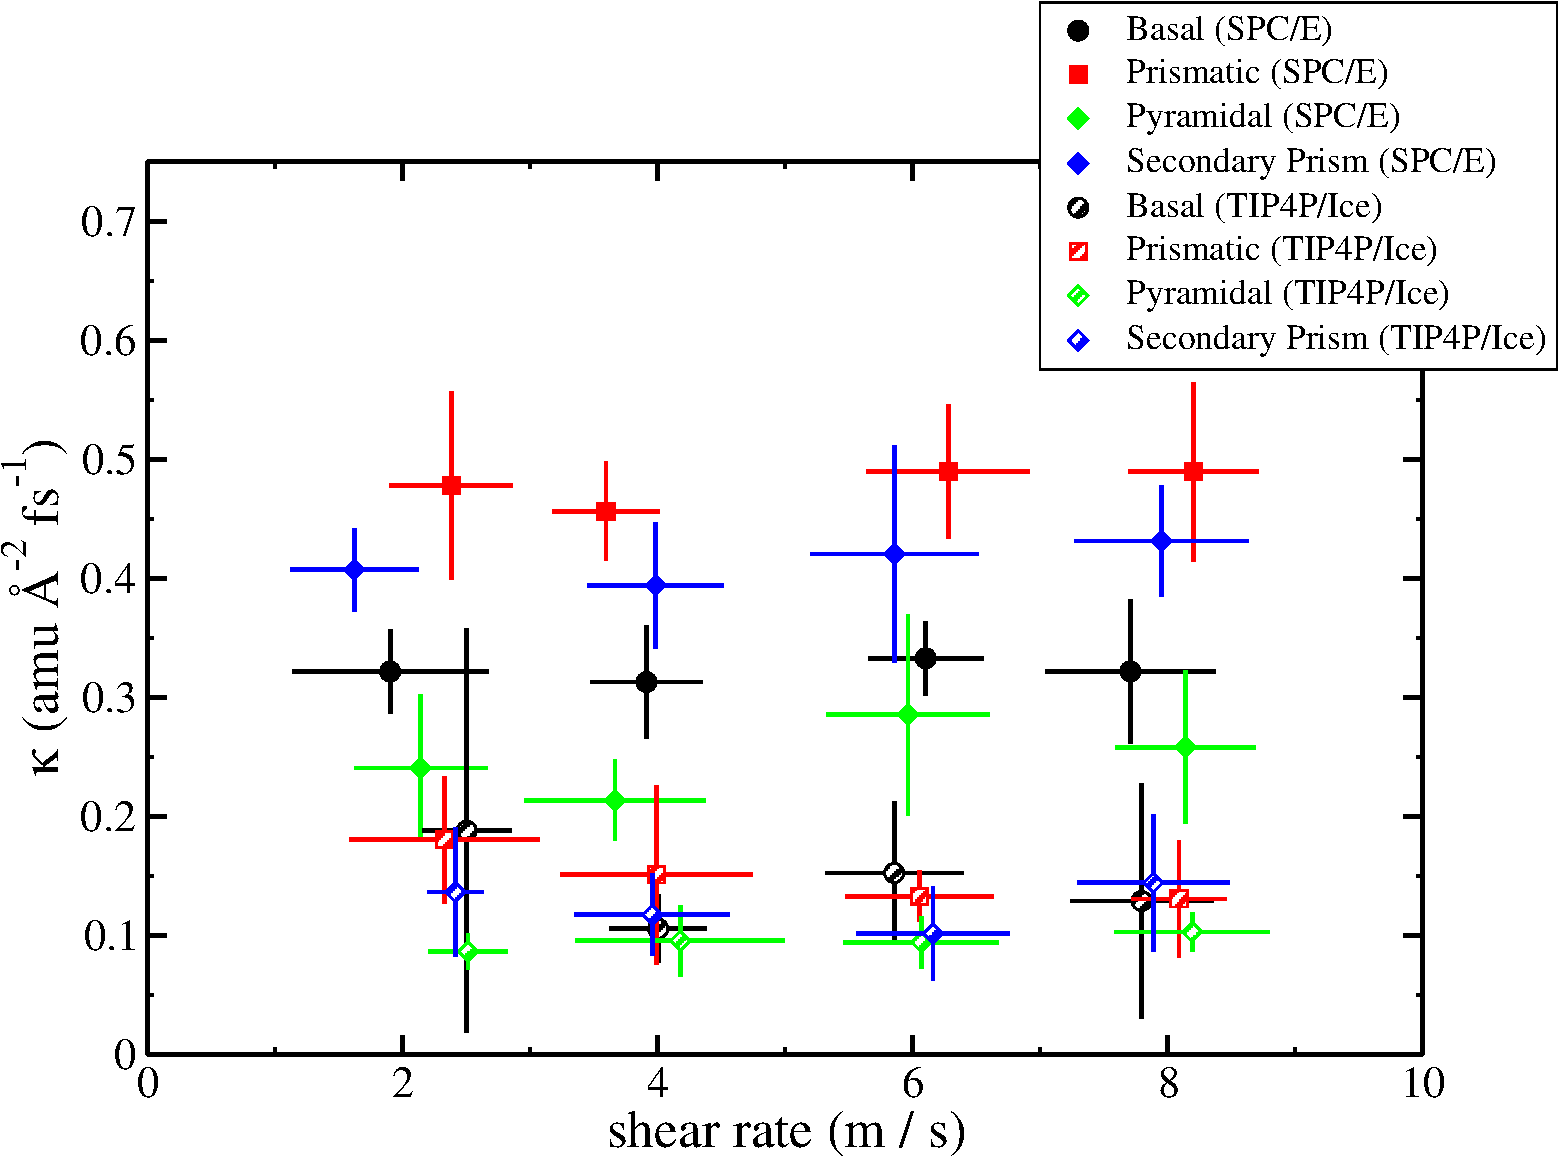
\includegraphics[width=\linewidth]{Figures/kappaPlot2}
\caption{\label{fig:kappaPlot} Dependence on the observed friction
  coefficient $\kappa$ on the shear rate of the ice through the surrounding
  liquid water.  The RNEMD simulations impose a momentum flux, but the
  resulting shear rates can vary.  Here, we collect data in 2 m/s bins
  to accumulate statistics over multiple independent simulations.  The
  SPC/E simulations (solid symbols) were done at 225~K, and the
  TIP4P/Ice simulations (patterned symbols) were carried out at
  270~K. The points on this plot have also been averaged over shear
  direction ($x$ and $y$).}
\end{figure}


\begin{table}[h]
\centering
\caption{SOLID / LIQUID FRICTION COEFFICIENTS ($\kappa$) FOR
  ICE-I$_\mathrm{h}$ INTERFACES WITH WATER \label{tab:kappa}}
\begin{tabular}{r|cc|cc}  
  \hline
\hline
  & \multicolumn{2}{c|}{SPC/E (225~K)} & \multicolumn{2}{c}{TIP4P/Ice (270~K)} \\
  Interface & $\kappa_{x}$ &  $\kappa_{y}$ & $\kappa_{x}$ &  $\kappa_{y}$ \\ 
  \hline
  Basal  $\{0001\}$                 & 0.32(5)  & 0.31(4) & 0.12(2)  & 0.13(2) \\
  Prismatic  $\{10\bar{1}0\}$       & 0.44(5)  & 0.46(5) & 0.16(2)  & 0.16(3) \\
  Pyramidal  $\{20\bar{2}1\}$       & 0.28(3)  & 0.25(3) & 0.09(1)  & 0.10(1) \\
  Secondary Prism  $\{11\bar{2}0\}$ & 0.44(4)  & 0.42(5) & 0.14(3)  & 0.14(2) \\ 
  \hline
\hline
\end{tabular}
\begin{flushleft}
  Friction coefficients $\kappa$ are measured in amu
  \AA\textsuperscript{-2} fs\textsuperscript{-1}, and uncertainties in
  the last digit are indicated with parentheses.
\end{flushleft}
\end{table}

Note that the values of $\kappa$ for the basal and prismatic crystal
facets in Table \ref{tab:kappa} disagree with values for interfacial
friction ($\lambda$) we previously in Table \ref{tab:lambda}. In our
preliminary investigation, the expression for the coefficient of
friction was derived from equation \eqref{eq:kappa1} and the linear
constitutive relation for shear stress in a bulk fluid.  However, as
described above, sheared ice / water interfaces are in the domain
negative slip lengths. Equation \eqref{eq:kappa1} should only be used in
slip boundary conditions, as negative slip can yield coefficients of
friction that appear to be smaller in magnitude than the zero slip
conditions. In our previous work, the prismatic surface was found to
have a larger negative slip length than the basal face, indicating a
prismatic surface that should have been reported with a larger
coefficient of friction. If one instead uses Equation \eqref{eq:Shenyu-13}
and interfacial widths to compute friction, the reported values come
into agreement.

The two water models give two significantly different values for the
friction coefficients. This is primarily a result of the difference in
water viscosities at the two coexistence temperatures ($\eta = $ 15.9
cP for SPC/E at 225~K and 6.1 cP for TIP4P/Ice at 270~K), which alters
the stream velocity on the liquid side of the interface. The relative
ratios of facet friction are similar in both models, however, with
$\kappa_\mathrm{prismatic} / \kappa_\mathrm{basal} =$ 1.56~(SPC/E) and
1.32~(TIP4P/Ice),
$\kappa_\mathrm{pyramidal} / \kappa_\mathrm{basal} =$ 0.84~(SPC/E) and
0.81~(TIP4P/Ice), and
$\kappa_\mathrm{secondary} / \kappa_\mathrm{basal} =$ 1.33~(SPC/E) and
1.15 (TIP4P/Ice). The observed ordering of facet friction
coefficients,
\begin{equation}
\kappa_\mathrm{pyramidal} < \kappa_\mathrm{basal} <
\kappa_\mathrm{secondary} < \kappa_\mathrm{prismatic} 
\end{equation} 
seems robust.

 
\section{Influences of Interfacial Friction}
The primary result presented in this chapter is the observation that
the different facets of ice-I$_\mathrm{h}$ produce significantly
different solid / liquid interfacial friction coefficients with water
(see Table \ref{tab:kappa}).  The two prismatic surfaces displayed the
largest coefficients of friction, while the basal and pyramidal facets
exhibited significantly lower friction. This trend is robust over a
wide range of shear rates, and shear direction relative to ice surface
features. Also, while the magnitude of the solid / liquid friction
coefficients differ due to liquid viscosities, the facet trends are
exhibited by both SPC/E and TIP4P/Ice at their coexistence
temperatures.

It is surprising that the observed solid / liquid friction
coefficients do not depend on the shear direction relative to surface
features. Pfalzgraff \textit{et al.} have recently investigated
diffusion of the water molecules comprising the quasi-liquid layer
(QLL) on the vacuum exposed basal, prismatic, and pyramidal surfaces
of an ice-I$_\mathrm{h}$ crystal.\cite{Pfalzgraff2011} They observed
anisotropic diffusion on the prismatic and pyramidal surfaces at 250~K
with the NE6 model ($\sim$~40~K below the melting temperature of that
model). In two following studies, Gladich \textit{et al.}
investigated the temperature dependence of this phenomena and deduced
the mechanism of anisotropic self-diffusivity at the prismatic
ice-vapor interface.\cite{Gladich2011,Gladich2015} They observed a
transition from anisotropic to isotropic diffusion at about 260~K with
the NE6 model, and attributed the transition to a change in the
prevailing mechanism of self-diffusion. At temperatures colder than
260~K, the QLL is sparse and the diffusing molecules are strongly
influenced by the underlying geometry of the crystal. At temperatures
warmer than 260~K, the QLL is thicker and diffusion occurs at the
outer part of the QLL. These results were robust for TIP4P/2005 and
TIP5P-Ew at the same relative undercooling temperature. Since our
ice-I$_\mathrm{h}$ / water interfaces are at their respective
coexistence temperatures, the effects of the underlying ice crystal
may be masked and we might expect to recover isotropic behavior.

The differences in friction are also surprising given that densities
and molecular interactions are identical for the four interfaces and
the interfacial widths measured via both structural and dynamic
features are also quite similar (for the interfaces treated with the
same water model). There are few remaining surface properties that
could give rise to differences in solid / liquid friction of the four
facets, notably surface corrugation, hydrogen bonding density, and
hydrogen bond lifetime at the interface. In this section we
investigate the roles of these surface features.

\subsection{Solid / Liquid Hydrogen Bond Density}
The four ice surfaces may potentially have different densities of
hydrogen bonds that bridge the solid and liquid. An ice surface that
forms more hydrogen bonds with the interfacial liquid would be able to
exert significant lateral forces on the liquid layer, yielding a
larger friction coefficient. To probe this possibility, we have
investigated the density of cross hydrogen bonds between the ice and
the liquid.

Quantifying water molecules as ``ice'' or ``liquid'' at an interface
of finite width requires a local order parameter for separating the
molecules.  Conde \textit{et al.}\cite{Conde2008} (and later Gladich
\textit{et al.}\cite{Gladich2011,Gladich2015}) discriminated molecules
as either ``ice'' or ``liquid'' by a threshold value of the local
tetrahedral order parameter (the same order parameter described here
in section \ref{sec:tetra}), denoted $q_{t}$. This threshold value was
obtained by equating the probability of incorrectly assigning a
liquid-like molecule as ice-like to the probability of incorrectly
assigning an ice-like molecule as liquid-like. Molecules with
$q < q_{t}$ were denoted as liquid-like, while those found having
$q > q_{t}$ were designated ice-like.

In a similar manner, we have chosen a threshold value of the local
tetrahedral order parameter as our partitioning criterion. Here,
$q_{t}$ is taken to be the value of the order parameter at the Gibbs
dividing surface ($q(z_0) \approx 0.84$ for SPC/E and
$q(z_0) \approx 0.85$ for TIP4P/Ice).  Note that some molecules have
strong tetrahedral ordering in the liquid phase, so this segregation
will not yield perfect division between ice and liquid phase
molecules.

To determine if a hydrogen bond has been formed between two water
molecules, we used the geometric criteria of Luzar and
Chandler.\cite{Luzar1996} We identify a hydrogen bond between two
water molecules if the distance between their oxygen sites,
$r_\mathrm{OO} < 3.5$~\AA, and the OHO bond angle,
$\theta_\mathrm{OHO} < 30^\circ$.

For each of the shearing simulations performed, a hydrogen bond
tetrahedrality matrix was constructed.  Snapshots from the shearing
trajectories were taken every $0.1$ ps, and the tetrahedrality $(q)$
value for each water molecule in the system was calculated. Hydrogen
bonds were also identified, and the tetrahedrality of the donor
$(q_{D})$ and acceptor $(q_{A})$ molecules were recorded. A
probability density of hydrogen bonds categorized by donor and
acceptor tetrahedrality, $\rho_\mathrm{HB}(q_D, q_A)$, was then
recorded.

\begin{figure}
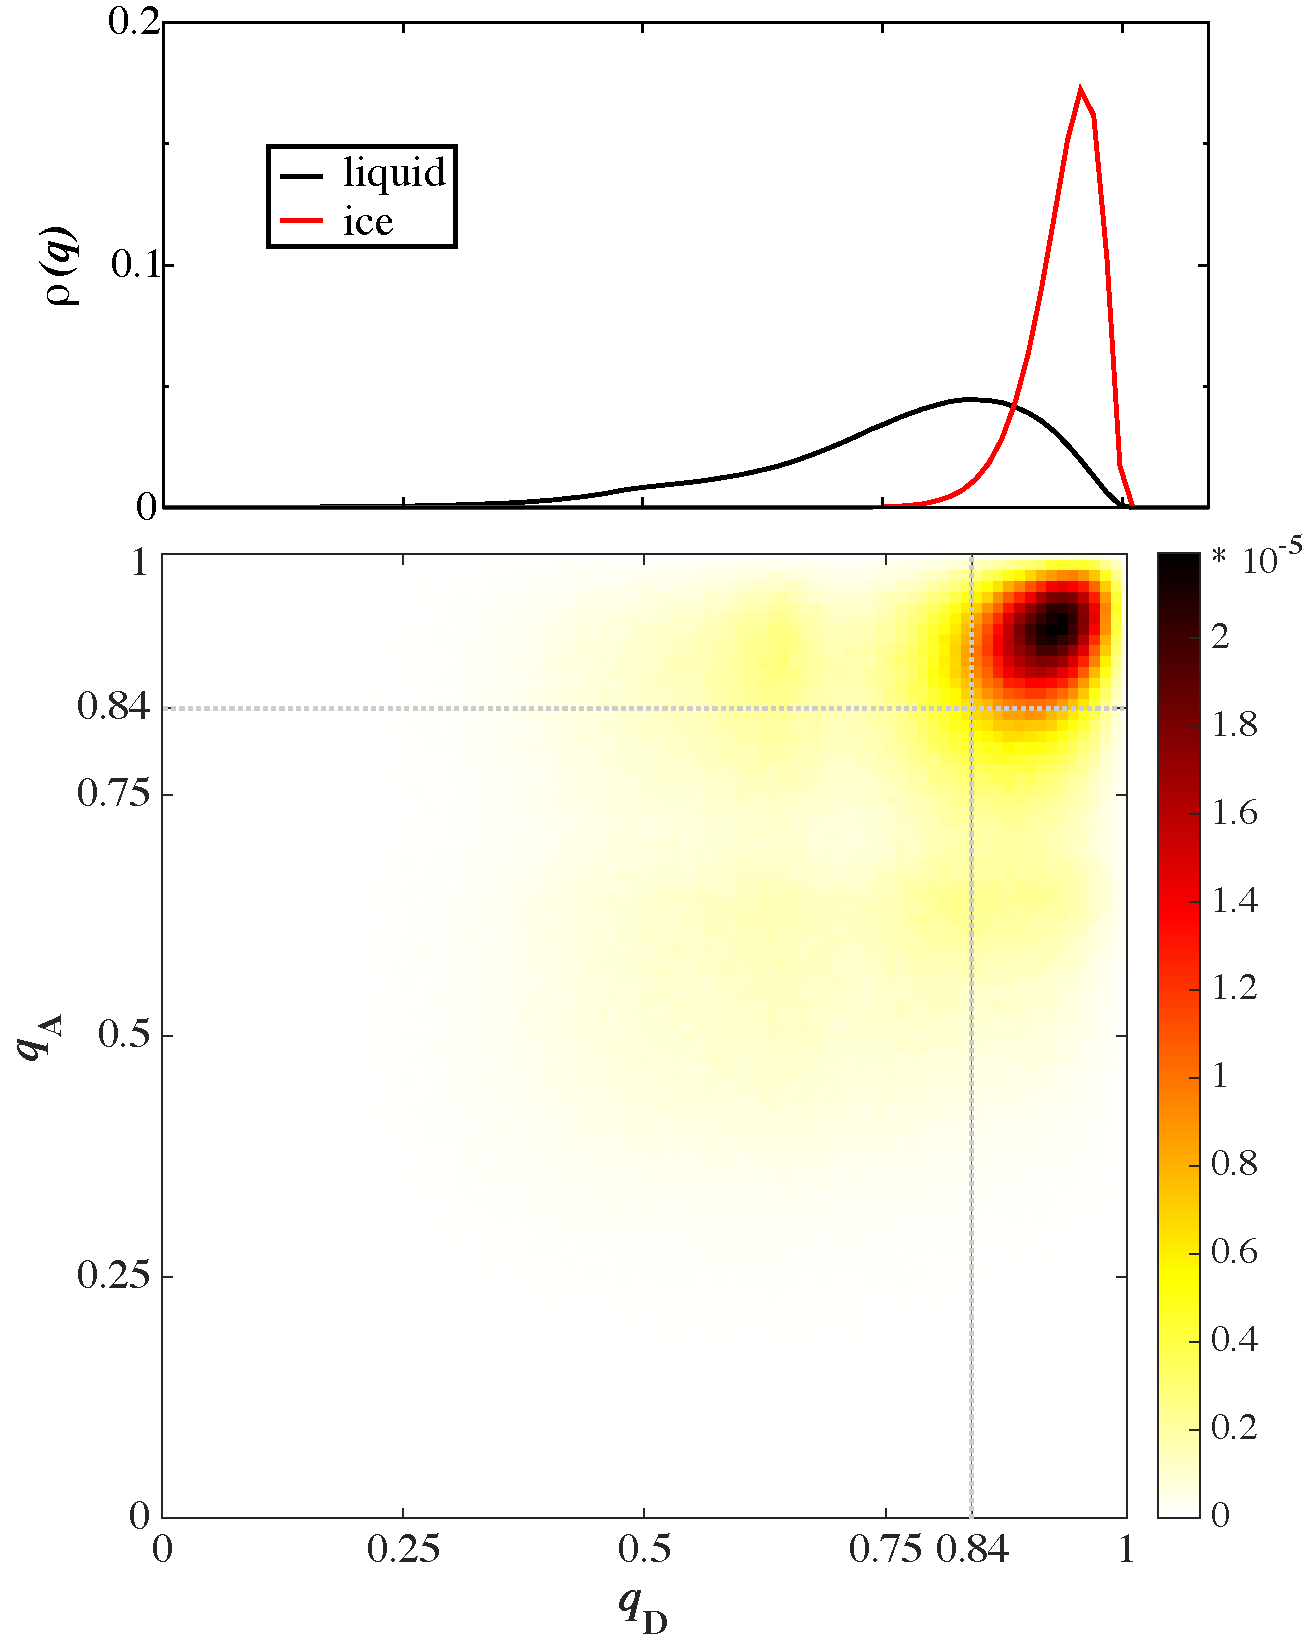
\includegraphics[width=5in]{Figures/hbtet.pdf}
\caption{\label{fig:tetHBMatrix} Distribution of hydrogen bonds at a
  prismatic interface showing the tetrahedralities of donor $(q_D)$
  and acceptor $(q_A)$ molecules (lower panel). Distributions of
  tetrahedralities in bulk ice and liquid phases are shown in the
  upper panel. The value of $q$ at the Gibbs dividing surface is
  indicated with dashed lines. Hydrogen bonds between ice molecules
  are represented by the upper right square, while those between
  liquid molecules are in the lower left.  Hydrogen bonds that bridge
  the ice-liquid interface exist primarily in the vertical and
  horizontal strips that remain.}
\end{figure}

The lower panel of Figure \ref{fig:tetHBMatrix} shows a hydrogen bond
tetrahedrality distribution for the prismatic facet with $q_{D}$
plotted along the $x$-axis and $q_{A}$ along the $y$-axis.  Population
around $q_{D} \approx q_{A} \approx 0.9$ indicates the density of
ice-ice hydrogen bonds in the system, while the liquid-state hydrogen
bonds are concentrated in the lower left, and are significantly more
diffuse.  The off-diagonal regions of the distribution represent the
population of molecules in tetrahedral (ice-like) environments bound
to non-tetrahedral (liquid-like) environments. Integrating the
population found in each of these regions and normalizing by the
surface area of each ice crystal produces a surface density of
hydrogen bonds (\AA\textsuperscript{-2}) formed between the ice and
interfacial liquid,
\begin{equation}\label{hbondDensity}
\rho_{sl} = \frac{N_\mathrm{HB}}{2 L_{x}L_{y}} \left[ \int_0^{q_{t}}
  dq_{D} \int_{q_{t}}^1 dq_{A}~\rho_\mathrm{HB}(q_{D},q_{A}) +  \int_0^{q_{t}}
  dq_{A} \int_{q_{t}}^1 dq_{D}~\rho_\mathrm{HB}(q_{D},q_{A}) \right]
\end{equation}
$N_\mathrm{HB}$ is the total number of hydrogen bonds found in the
system, and $L_x$ and $L_y$ are the dimensions of the two ice facets
exposed to the liquid.  Values for $\rho_{sl}$ for each of the ice
surfaces are reported in Table \ref{tab:hbondDens}.

\begin{table}[h]
\centering
\caption{ SURFACE HYDROGEN BOND DENSITIES FOR SPC/E AND
  TIP4P/Ice MODELED ICE-I$_\mathrm{h}$ / WATER INTERFACES \label{tab:hbondDens}} 
\begin{tabular}{r|c|c}  
  \hline
\hline
  & \multicolumn{1}{c|}{SPC/E (225~K)} & TIP4P/Ice (270~K) \\
  Interface & $\rho_{sl}$ (\AA\textsuperscript{-2}) & $\rho_{sl}$ (\AA\textsuperscript{-2}) \\ 
  \hline
  Basal  $\{0001\}$                 & 0.1227(3) & 0.0749(9) \\
  Prismatic  $\{10\bar{1}0\}$       & 0.2014(5) &  0.141(1) \\
  14\degree~Pyramidal  $\{20\bar{2}1\}$       & 0.0866(3) & 0.074(1) \\
  Secondary Prism  $\{11\bar{2}0\}$ & 0.1384(4) & 0.119(1) \\ 
  \hline
\hline
\end{tabular}
\begin{flushleft}
Uncertainties in the last digit are indicated with
  parentheses.
\end{flushleft}
\end{table}



The trend in surface density of solid / liquid hydrogen bonds
reproduces the trend in the friction coefficients, indicating that
friction at ice-I$_\mathrm{h}$ water interfaces is strongly influenced
by the number of solid / liquid hydrogen bonds that can be formed.
This result is robust under multiple shear rates and orientation of
shear flow relative to the surface features of the ice (that is, shear
in both the $x$ and $y$ dimensions), indicating that the hydrogen
bonding statistics between an ice facet and the liquid are not altered
by the imposed shear.

\subsection{Surface Corrugation by Projected Densities}
A second possible influence on the friction coefficient is the surface
topography of the ice crystals. To investigate this possibility, we
computed the mean projected density ($\rho(y,z)$),
\begin{equation}
\rho(y, z) = \frac{1}{L_x~dy~dz} \left< \sum_{i = 1}^{N} m_i \delta(y_i - y) \delta(z_i - z)\right>
\end{equation}
for four quiescent interfaces over 1 ns of simulation time (sampled
every 1 ps).  Here, $dy$ and $dz$ are the lengths and widths of a set of
parallelepipeds that span the box depth ($L_x$), and for relatively
small $dy$ and $dz$ (0.05 \AA), the parallelepiped densities show the
smooth transition between the ordered ice facet and the surrounding
liquid.

\begin{figure}
\includegraphics[width=\linewidth]{Figures/DensityPlots}
\caption{\label{fig:DensPlots} Projected densities, $\rho(y, z)$, at
  the four quiescent interfaces.  Darker colors represent higher
  densities, while lighter colors (e.g. white) are relatively
  unpopulated.  For all four interfaces, the location of the
  tetrahedrality Gibbs dividing surface is indicated with a solid
  black line, while the two end points of the 10-90 width are shown in
  grey.}
\end{figure}

We note that the projected densities allow computation of the channel
widths and depth for the two prismatic facets using the locations of
the peak densities.  These figures also indicate that below the Gibbs
dividing surface, almost no liquid state molecules can be found
occupying the channels.  The structure of the surface corrugation can
be obtained by measuring the peak-to-peak distances of the
liquid-exposed crystal structures, the dimensions of which are
reported in Table \ref{tab:surf}. When a crystal of ice-I$_\mathrm{h}$
is cleaved along either of the two prismatic crystal facets, the
exposed oxygen atoms present channel-like structures with channel
widths of $\sim$ 5~\AA~ and channel depths of $\sim$ 2.3~\AA~.  When
cleaved along the pyramidal facet, the resulting surface features a
much larger channel, $\sim$ 8.3~\AA~ wide.  Conversely, the basal
surface presents a rather smooth surface to the liquid, with stripes
of oxygen atoms forming surface ripples with depths of $\sim$ 1~\AA~.

\begin{table}[h]
\centering
\caption{SURFACE FEATURES OF ICE-I$_\mathrm{h}$ FACETS\label{tab:surf}}
\begin{tabular}{r|cc}  
\hline
\hline
Interface & Channel width (\AA) & Channel depth (\AA) \\ 
\hline
Basal  $\{0001\}$                 & 3.5(2) & 0.9(1)  \\
Prismatic  $\{10\bar{1}0\}$       & 4.5(1) & 2.4(3)  \\
14\degree~Pyramidal  $\{20\bar{2}1\}$       & 8.3(2) & 1.9(4)  \\
Secondary Prism  $\{11\bar{2}0\}$ & 5.3(4) & 2.2(1)  \\ 
\hline
\hline
\end{tabular}
\end{table}

The prismatic channels are quite stable. That is, the projected
density in the prismatic and secondary prism surface channels is small
relative to the bulk liquid density $(\rho(y,z) < \rho_l / 7)$.  One
might expect regions of low liquid density to yield smaller solid /
liquid interactions, and it does appear that these two surfaces
present roughly half of the surface oxygen atoms to the liquid.
However, the molecules forming the bottoms of the channels are fully
saturated (four hydrogen bonds each), while the molecules that form
the tops of the channels present a high density of available hydrogen
bond locations.

The oxygen-based surface features of the prism and secondary prism are
similar, and only the orientation of the water molecules varies.  This
means that the patterning of donor and acceptors on the two facets is
quite different. A liquid with internal hydrogen bonding constraints
that is in contact with these facets will allow the prismatic surface
to form a higher density of solid / liquid hydrogen bonds than the
secondary prism, even with identical oxygen ordering at the interface.

% In contrast with the prismatic facets, liquid state molecules can
% populate the surface channels on the pyramidal facet. Again, one might
% expect the interactions between the solid and the liquid in close
% physical contact to be quite large.  However, the liquid molecules
% populating this channel do not pack efficiently and cannot fully
% saturate the surface locations available for hydrogen bonding,
% resulting in a lower solid / liquid hydrogen bond density and a
% smaller coefficient of friction.

With its smooth surface, one could make reasonable physical arguments
for the basal face to have either high or low friction with liquid
water. That is, liquid molecules should be able to form a fully
populated network of hydrogen bonds with the surface, as there are no
recessed surface molecules at the bottoms of deep channels. In the
absence of large surface undulations, however, liquid-phase molecules
should also be able to slip over the surface easily. However, the
basal facet was found to have an intermediate friction coefficient
compared with the other facets studied here. The sensible explanation
in light of the hydrogen bonding data is simply that the surface
density of solid / liquid hydrogen bonds (however transitory)
dominates the interfacial friction.

\subsection{Hydrogen Bond Lifetime at the Interface}
A third possible influence to the friction at the ice-I$_\mathrm{h}$ /
water interface is that there are differential lifetimes of hydrogen
bonds for the crystal facets investigated. A crystal face with longer
persisting hydrogen bonds would impose more drag on the liquid, which
could result in a larger friction coefficient. 

In order to determine the lifetime of the hydrogen bond, we can
investigate the hydrogen bond jump rate at the interface. In Chapter
\ref{chap:Dyn} we discussed how the hydrogen bond jump rate was
calculated, and the results are presented in
Figure \ref{fig:SPCEjumpRates} and Figure \ref{fig:TIP4PIcejumpRates}. By
querying the value of $k_\mathrm{jump}^{-1}$ at each interface, we
have obtained estimates of the hydrogen bond lifetime for each of the
crystal facets under the two models. Here, we have obtained
$\tau_{HB}$ at the interface as determined by both the local
tetrahedral order parameter, and as determined by the jump rates ;
these values are reported in Table \ref{tab:jumpRates}.


\begin{table}[h]
\centering
\caption{HYDROGEN BOND LIFETIMES  ($k_\mathrm{jump}^{-1}$) FOR
  ICE-I$_\mathrm{h}$ / WATER INTERFACES\label{tab:jumpRates}}
\begin{tabular}{r|cc|cc}  
\hline
\hline
& \multicolumn{2}{c|}{SPC/E (225~K)}  &
                                                  \multicolumn{2}{c}{TIP4P/Ice
                                        (270~K)}  \\ 
Interface & $q_\mathrm{mid}$ & $j_\mathrm{mid}$ & $q_\mathrm{mid}$
                              & $j_\mathrm{mid}$ \\
\hline
Basal  $\{0001\}$                 & 500 & 111 & 111 & 50 \\
Prismatic  $\{10\bar{1}0\}$       & 333 & 167 & 143 & 50 \\
14\degree~Pyramidal  $\{20\bar{2}1\}$       & 500 & 100   & 125 & 50\\
Secondary Prism  $\{11\bar{2}0\}$ & 333 &111  & 100 & 50\\ 
\hline
\hline
\end{tabular}
\begin{flushleft}
Hydrogen bond lifetimes measured at the structural interface (as
determined by tetrahedrality) and at the dynamic interface (as
measured by hydrogen bond jump time) are reported in ps.
\end{flushleft}
\end{table}

We find that the lifetime of hydrogen bonds at the structural SPC/E
ice-I$_\mathrm{h}$ / water interface has a lifetime of $\sim$ 500 ps
for the basal and pyramidal facets, and about 300 ps for the two
prismatic facets. This is significantly longer than compared with the
lifetime obtained when querying at the midpoint of the hydrogen bond
jump interface, which estimates the lifetime to be about 100 ps for
each of the interfaces. Here, the prismatic surface displays a
slightly longer lifetime than the other three facets.  The TIP4P/Ice /
water interfaces have significantly shorter lived hydrogn bonds, with
lifetimes of about 100 ps at the structural interface and 50 ps at the
hydrogen bond jump interface. For all interfaces, the hydrogen bond
lifetime is observed to be longer-lived in the SPC/E interfaces as
compared to the TIP4P/Ice interfaces. This is primarily due to the
warmer coexistence temperature for the TIP4P/Ice model, leading to
faster dynamics of the water molecules. However, there is no observed
trend in the lifetime of the hydrogen bonds with the observed
friction, further indicating that friction at ice-I$_\mathrm{h}$ /
water interfaces is governed by the density of solid / liquid hydrogen
bonds.

\section{A Simple Model For Solid-Liquid Friction}
The interfacial friction coefficient, $\kappa$ captures the momentum
conductance transverse to the interface, and this momentum should be
transferred via strong intermolecular interactions across the
interface. This is measured in ice-I$_\mathrm{h}$ / water systems by
the surface density of hydrogen bonds, $\rho_\mathrm{s-l}$.  The
momentum is then carried through the liquid via viscous forces
$(\eta)$ across an interfacial region that has width
$w_\mathrm{s-l}$. A simple linear model,
\begin{equation}
  \kappa = c~~\rho_\mathrm{s-l}~~\eta~~w_\mathrm{s-l},
\label{eq:model}
\end{equation}
captures these features at the ice-I$_\mathrm{h}$ / water interface,
and the results for the two water models nearly coalesce with a
proportionality constant, $c = 0.343$ (see
Figure \ref{fig:simpleModel}).  The structural width,
$w_\mathrm{10-90}^{q}$, and values for $\eta$ for each ice / water
system were obtained by fitting the liquid portions of the simulation
box in conjunction with equation \eqref{eq:viscosity}.  The two water
models have two different coexistence temperatures, so they exhibit
different hydrogen bond densities and viscosities adjacent to the
interface.  Comparing Equation \eqref{eq:model} with the non-equilibrium
expressions for $\kappa$ (Equation \eqref{eq:Shenyu-13}) and $\eta$
(Equation \eqref{eq:viscosity}) shows that the liquid's viscosity is an
important feature in capturing the velocity drop on the liquid side of
the interface ($\eta w_\mathrm{s-l}$), but the magnitude of the
solid-liquid interactions ($c~~\rho_\mathrm{s-l}$) plays a central
role in the observed friction.

\begin{figure}
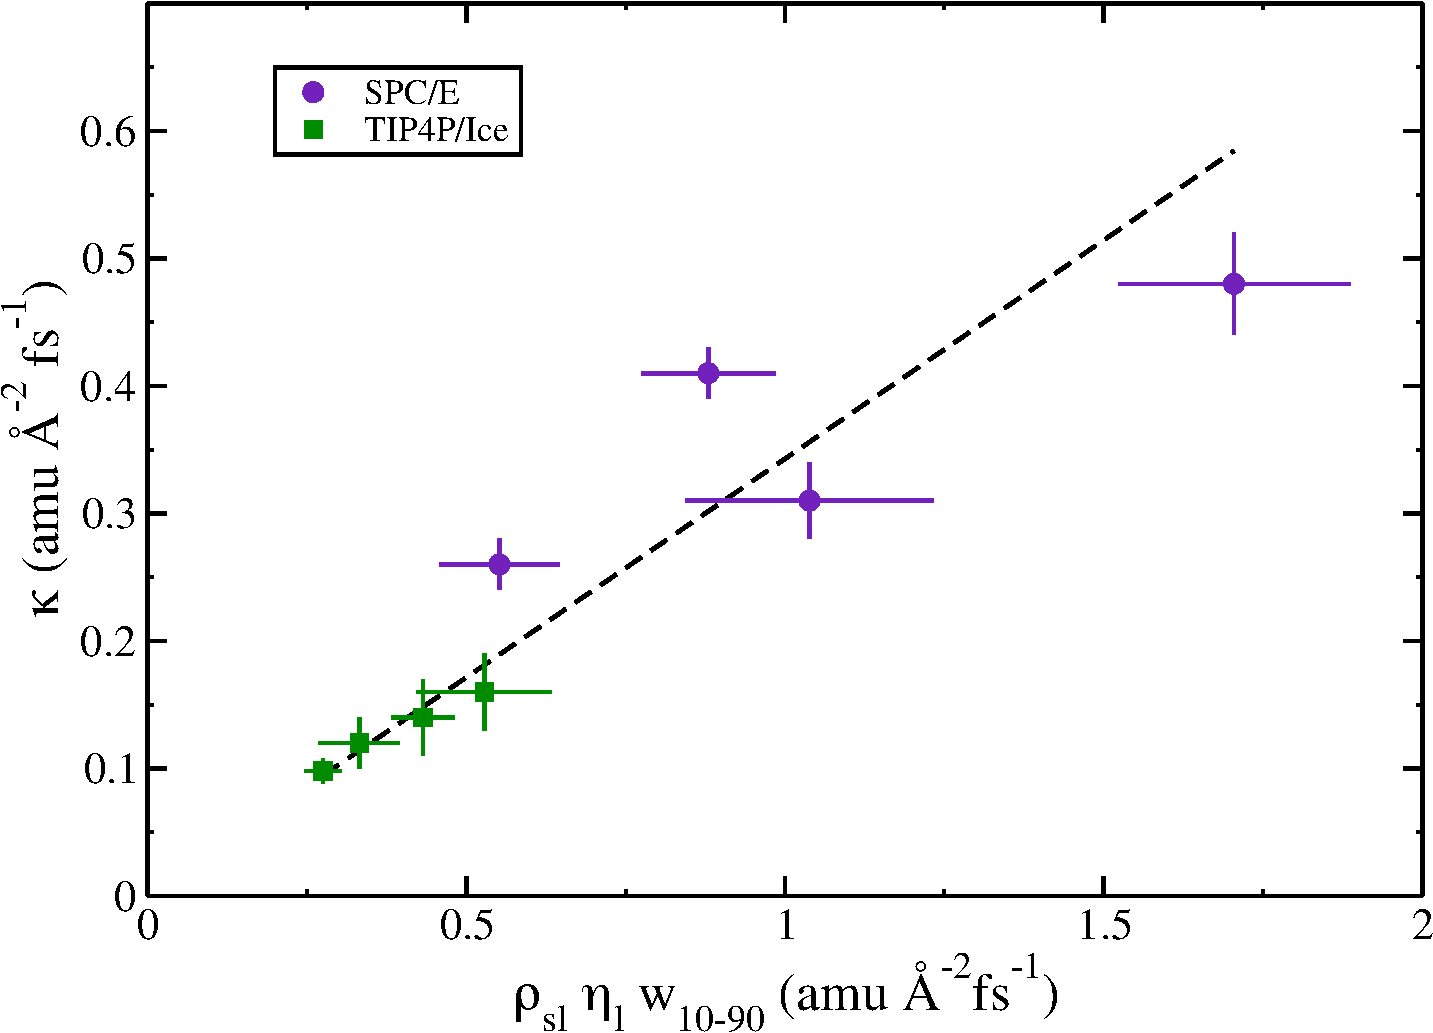
\includegraphics[width=\linewidth]{Figures/simpleModel}
\caption{\label{fig:simpleModel} Solid-liquid friction coefficients
  shown vs. surface hydrogen bond density model (Equation \eqref{eq:model})
  for all four facets and for both water models.  Although SPC/E
  (225K) and TIP4P/Ice (270K) operate in two distinct viscosity
  domains, the model captures the importance of the density of
  solid-liquid hydrogen bonds.}
\end{figure}                                            

\section{Summary}
RNEMD simulations of the different facets of ice being drawn through
surrounding water at the coexistence temperature indicate
facet-dependence of solid / liquid friction.  We have defined a
negative slip interfacial friction coefficient, $\kappa$ (measured in
amu~\AA$^{-2}$ fs$^{-1}$) and find that the two prismatic facets exert
the largest drag on the surrounding liquid.  The basal facet provides
an intermediate level of drag, while the pyramidal facet has roughly
half the interfacial friction of the prismatic facet.

Using the local tetrahedral order parameter as a metric to
differentiate ice and liquid water molecules and a geometric hydrogen
bonding criteria, the friction coefficients were shown to be largely
governed by the surface density of solid / liquid hydrogen bonds
($\rho_{sl}$).  A simple linear model, Equation \eqref{eq:model}, uses
this density to provide estimates of solid-liquid friction that give
good agrement for two different water models at their respective
coexistence temperatures.

In Chapters \ref{chap:Str} and \ref{chap:Dyn}, we presented evidence
that the ice-I$_\mathrm{h}$ / water interfacial widths for all four
crystal facets are similar (using both structural and dynamic
measures) and found these widths to be independent of shear rate.  The
similarity of interfacial width estimates for the four facets indicate
that the particular facet of the exposed ice crystal has very little
effect on how far into the bulk the ice-like structural ordering
persists. While differences have been found in previous simulations of
ice-I$_\mathrm{h}$ / water interfaces,\cite{Hayward2001,Hayward2002}
experimentally these differences have been less
clear.\cite{Beaglehole1993} The significant differential friction
coefficients obtained here suggest that while the liquid next to the
ice might be structurally organized like bulk liquid, the dynamics of
the molecules are still quite strongly perturbed by the ice.  That is,
the surface hydrogen bonding significantly alters how the water layers
are pulled along with the ice during shear.


